%% 
%% Copyright 2007-2019 Elsevier Ltd
%% 
%% This file is part of the 'Elsarticle Bundle'.
%% ---------------------------------------------
%% 
%% It may be distributed under the conditions of the LaTeX Project Public
%% License, either version 1.2 of this license or (at your option) any
%% later version.  The latest version of this license is in
%%    http://www.latex-project.org/lppl.txt
%% and version 1.2 or later is part of all distributions of LaTeX
%% version 1999/12/01 or later.
%% 
%% The list of all files belonging to the 'Elsarticle Bundle' is
%% given in the file `manifest.txt'.
%% 
%% Template article for Elsevier's document class `elsarticle'
%% with harvard style bibliographic references

%\documentclass[preprint,12pt,authoryear]{elsarticle}

%% Use the option review to obtain double line spacing
%% \documentclass[authoryear,preprint,review,12pt]{elsarticle}

%% Use the options 1p,twocolumn; 3p; 3p,twocolumn; 5p; or 5p,twocolumn
%% for a journal layout:
%% \documentclass[final,1p,times,authoryear]{elsarticle}
%% \documentclass[final,1p,times,twocolumn,authoryear]{elsarticle}
%% \documentclass[final,3p,times,authoryear]{elsarticle}
\documentclass[final,3p,times,twocolumn,numbers]{elsarticle}
%% \documentclass[final,5p,times,authoryear]{elsarticle}
%% \documentclass[final,5p,times,twocolumn,authoryear]{elsarticle}

%% For including figures, graphicx.sty has been loaded in
%% elsarticle.cls. If you prefer to use the old commands
%% please give \usepackage{epsfig}

%% The amssymb package provides various useful mathematical symbols
\usepackage{amssymb}
%% The amsthm package provides extended theorem environments
\usepackage{amsthm}

\usepackage{mhchem}
\usepackage{xcolor}
\usepackage{csvsimple,booktabs}


\usepackage{algorithm}
\usepackage{algorithmicx}
\usepackage{algpseudocode}

%% The lineno packages adds line numbers. Start line numbering with
%% \begin{linenumbers}, end it with \end{linenumbers}. Or switch it on
%% for the whole article with \linenumbers.
%% \usepackage{lineno}

\journal{Applied Energy}

\begin{document}

\begin{frontmatter}

%% Title, authors and addresses

%% use the tnoteref command within \title for footnotes;
%% use the tnotetext command for theassociated footnote;
%% use the fnref command within \author or \address for footnotes;
%% use the fntext command for theassociated footnote;
%% use the corref command within \author for corresponding author footnotes;
%% use the cortext command for theassociated footnote;
%% use the ead command for the email address,
%% and the form \ead[url] for the home page:
 \title{Validating the long-term electricity market model ElecSim using genetic algorithms}
% \tnotetext[label1]{}
 \author{Alexander J. M. Kell}
 \ead{a.kell2@newcastle.ac.uk}
% \ead[url]{home page}
% \fntext[label2]{}
% \cortext[cor1]{}
% \address{Address\fnref{label3}}
% \fntext[label3]{}

%\title{Validating a long-term electricity market model}

%% use optional labels to link authors explicitly to addresses:
%% \author[label1,label2]{}
%% \address[label1]{}
%% \address[label2]{}

\author{A. Stephen McGough, Matthew Forshaw}

\address{School of Computing, Newcastle University, Newcastle-upon-Tyne, United Kingdom}

\begin{abstract}
%% Text of abstract

\end{abstract}
%
%%%Graphical abstract
%\begin{graphicalabstract}
%\includegraphics{grabs}
%Hello test
%\end{graphicalabstract}
%
%%%Research highlights
%\begin{highlights}
%\item Validating a model
%\item Optimisation
%\item Scenario modelling
%\end{highlights}

\begin{keyword}
%% keywords here, in the form: keyword \sep keyword
Long-Term Energy Modelling \sep Model Validation \sep Machine learning \sep Optimization \sep Climate Change
%% PACS codes here, in the form: \PACS code \sep code

%% MSC codes here, in the form: \MSC code \sep code
%% or \MSC[2008] code \sep code (2000 is the default)

\end{keyword}

\end{frontmatter}

%% \linenumbers

%% main text
\section{Introduction}
\label{sec:intro}


To limit the effects of climate change, a transition from a fossil-fuel based energy system to one based on low-carbon, renewable energy is required. The report by the Intergovernmental Panel on Climate Change detailed that reaching and sustaining zero global anthropogenic \ce{CO2} would halt anthropogenic global warming on multi-decadal time scales \cite{Masson-Delmotte2018}. 

The Paris Agreement was a declaration signed in 2015 by 195 state parties to plan and regularly report on the contribution made to mitigate global warming \cite{May2002}. Based on this commitment, policy makers require quantitive advice on interventions to aid in the mitigation of climate change and limit global average temperatures to well below 2$^{\circ}$C. 

The decarbonization of electricity generation is of strategic importance for this goal due to the fact that low-carbon electricity can enable reductions in \ce{CO2} emissions in industry, transport and building sectors~\cite{Salas2017}. 

However, there remain a number of uncertainties in the technological transition to a low-carbon energy supply. Examples of these uncertainties are investor behaviour, future prices of electricity generation and storage, domestic and international policy, energy efficiency and electricity demand. To successfully create effective policies an increase in understanding of these uncertainties and how they interact is required.

Energy modelling is a method that allows policy makers to increase their understanding of policy decision outcomes under a wide range of scenarios. Agent-based modelling (ABM) is a simulation technique that allows for heterogeneous agents to interact and can lead to effects on the aggregated level of the total system, a phenomenon called ``emergence'' \cite{EpsteinJoshuaM.author.GSSS}. Traditional models for analysing electricity systems, such as centralised optimisation models do not account for the heterogeneous nature of electricity investors and are, to some extent, based on obsolete assumptions~\cite{Ringler2016}.

In this paper we motivate that agent-based models are a valid way of complimenting existing models to provide advice to decision makers. We show that the model ElecSim \cite{Kell} can be validated over a 5 year period, starting from the year 2013 and ending in the year 2018, with a root mean squared error of {\color{red} $\sim0.045$} and a standard deviation of {\color{red}$\sim0.16$}. Similarly to Nahmmacher \textit{et al.} we demonstrate how clustering of multiple relevant time series such as electricity demand, solar irradiance and wind speed can reduce computational time by selecting representative days~\cite{Nahmmacher2016}. However, distinctly to Nahmacher \textit{et al.} we use a K-means clustering approach \cite{forgy65} as opposed to a hierarchical clustering algorithm described by Ward \cite{doi:10.1080/01621459.1963.10500845}.

We use a genetic algorithm approach to find an optimal set of price curves predicted by generation companies (GenCos) that  adequately model observed investment behaviour in the real-life electricity market in the United Kingdom. However, similar techniques can be employed for other countries of various sizes \cite{Kell}. We are able to model the transitional dynamics of the electricity mix in the United Kingdom as shown in Figure \ref{fig:uk_historical_mix}, where there was an $\sim88\%$ drop in coal use, $\sim44\%$ increase in Combined Cycle Gas Turbines (CCGT), $\sim111\% $ increase in wind energy and increase in solar from near zero to $\sim 1250$MW.


\begin{figure}
\centering
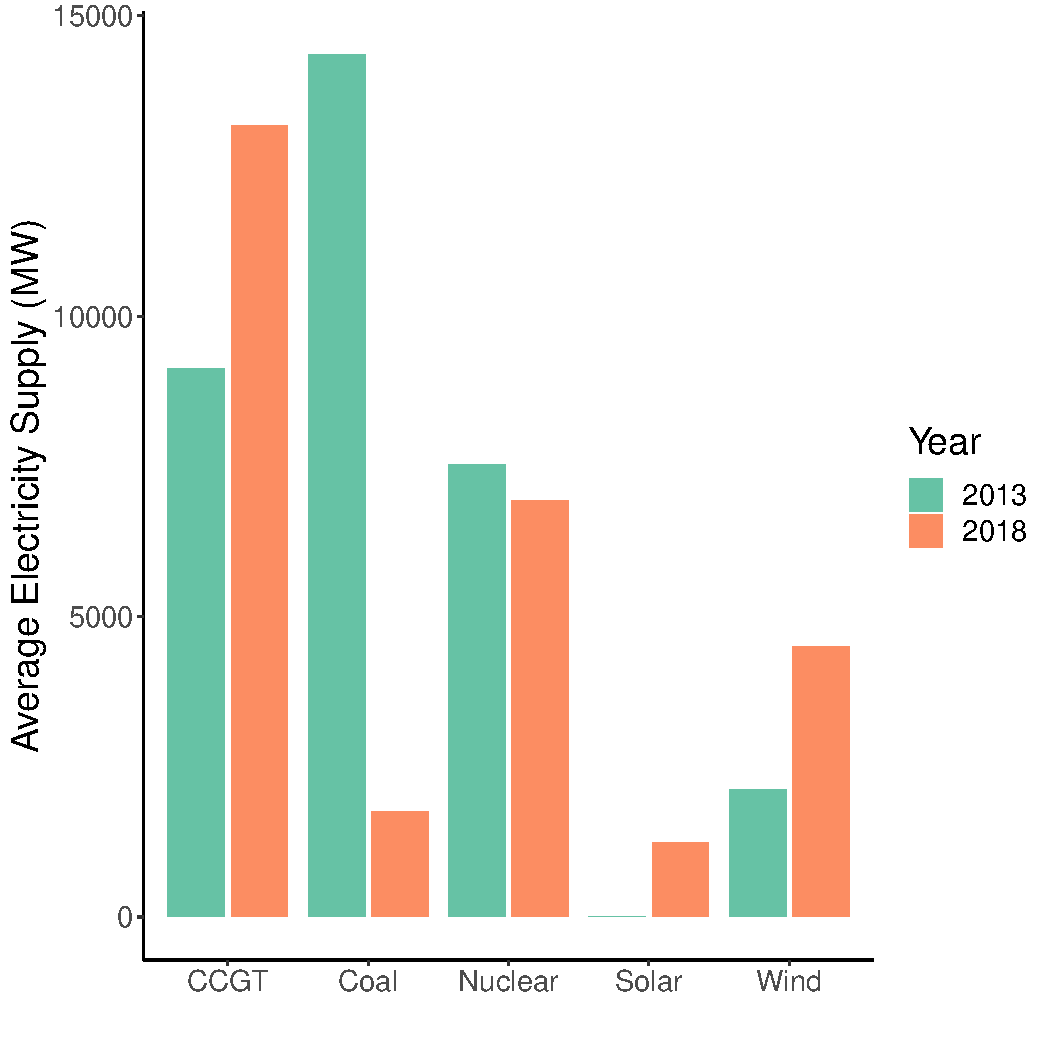
\includegraphics[width=0.46\textwidth]{figures/introduction/uk_historical_mix.pdf}
\caption{Electricity generation transition from 2013 to 2018 in the United Kingdom.}
\label{fig:uk_historical_mix}
\end{figure}

There is a desire to validate the ability of energy-models to make long-term predictions. Validation increases confidence in the outputs of a model and leads to an increase in trust amongst the public and policy makers. However, energy models are frequently criticised for being insufficiently validated, with the performance of models rarely checked against historical outcomes \cite{Beckman2011}.

The model OSeMOSYS \cite{Howells2011} is, however, validated against the similar model MARKAL\slash TIMES through the use of a case study named UTOPIA which is a simple test energy system bundled with ANSWER, a graphical user interface packaged with the MARKAL model generator \cite{Hunter2013, Noble2004}. Hunter \textit{et al.} use the same case study to validate their model Temoa \cite{Hunter2013}. Whereas the model PowerACE shows that realistic prices are achieved through modelling, however do not indicate success in modelling investor behaviour \cite{Ringler2012}.

Under the definition by Hodges \textit{et al.} \cite{Hodges}, however, long-range energy forecasts are not validatable \cite{Craig2002}. Under this definition, validatable models must be observable, exhibit constancy of structure in time, exhibit constancy across variations in conditions not specified in the model and it must be possible to collect ample data \cite{Hodges}.

Whilst it is possible to collect data for energy models, the data covering important characteristics of energy markets are not always measured. Furthermore, the behaviour of the human population and innovation are neither constant or entirely predictable. This leads to the fact that static models cannot keep pace with global long-term evolution. Assumptions made by the modeller may be challenged in the form of unpredictable events, such as the oil shock of 1973.

This, however, does not mean that energy-modelling is not useful for providing advice in the present. A model may fail at predicting the long-term future because it has forecast an undesirable event, which lead to a change in human behaviour. Thus avoiding the original scenario that was predicted, and can be viewed as a success of the model.

Work by Koomey \textit{et al.} expresses the importance of conducting retrospective studies to help improve models \cite{Koomey2003}. For example, a model can be rerun using historical data in order to determine how much of the error in the original forecast resulted from structural problems in the model itself and how much from incorrect specification of the fundamental drivers of the forecast \cite{Koomey2003}.

A retrospective study published in 2002 by Craig \textit{et al.} focused on the ability for forecasters to accurately predict electricity demand from the 1970s \cite{Craig2002}. They found that actual energy usage in 2000 was at the very lowest end of the forecasts, with only one exception. They found that these forecasts underestimated unmodelled shocks such as the oil crises which lead to increased energy efficiency.

Hoffman \textit{et al.} also developed a retrospective validation of a predecessor of the current MARKAL\slash TIMES model named Reference Energy System \cite{Hoffman_1973}, and the Brookhaven Energy System Optimization Model \cite{ERDA_48}. These were studies applied in the 70s and 80s to develop projections to the year 2000 . They found that the models were able to be descriptive, but were not entirely accurate in terms of predictive ability. They found that emergent behaviours in response to policy had a strong impact on forecasting accuracy. They concluded that forecasts must be expressed in highly conditioned terms \cite{Hoffman2011}. 

Schurr \textit{et al.} argued against predicting too far ahead in energy modelling due to the uncertainties involved \cite{Schurr_1961}. However, they specify that long-term energy forecasting is useful to provide basic information on energy consumption and availability which is helpful in public debate and in guiding policy makers.


Ascher concurs with this view, and states that the most significant factor in model accuracy is the time horizon of the forecast, with the more distant the forecast target, the less accurate, due to unforeseen changes in society as a whole ~\cite{gillespie_1979}.

It is for the reasons previously described that this paper focuses on a shorter-term (5 year) horizon window when validating the model. This enabled us to increase confidence that the dynamics of the model worked without external shocks and could provide descriptive advice to stakeholders.


%\begin{itemize}
%	\item Energy systems modelling to help transition to low-carbon energy systems (Paris Agreement)
%	\item Application of quantitive analysis to policy
%	\item Use of agent-based models to model heterogeneous actors
%	\item Optimum policy interventions for a smooth transition
%	\item Requirement to validate model using historical data
%	\item Prediction of electricity prices to understand optimal decisions
%	\item Confidence in model under certain scenarios
%\end{itemize}



\section{Material and methods}
\label{sec:methods}

The model, ElecSim, is made up of five distinct sections: power plant data; scenario data; the time-steps of the algorithm; the power exchange and the investment algorithm. ElecSim has been previously published \cite{Kell}, however, amendments have since been made to the model in the form of efficiency improvements as well as increasing the granularity of time-steps from yearly to representative days. In this paper we have used 8 representative days for electricity demand, solar irradiance and offshore and onshore wind speed. Each representative day was made up of hourly time-steps (24 time-steps per day).

In this section we summarize previously published results and detail the modifications made for this paper. In this paper we initialised the model to a scenario of the United Kingdom, however, the model is generalisable to any country and is dependent on input data.

\subsection{Plant Data}

The simulation was initialised with every power plant and generation company (GenCo) in the United Kingdom using a Department of Business, Energy and Industrial Strategy (BEIS) of the British government DUKES dataset for the year 2013 \cite{dukes_511}. The individual costs of these power plants were also initialised with data from the Department of Business, Energy and Industrial strategy of the British government \cite{Department2016}. For power plants that were out of the scope of this dataset (pre-2018), historical levelized cost of electricity (LCOE) values were used to infer the granular costs by a scaling factor from the International Energy Agency (IEA)~\cite{IEA2015}. Historical efficiency was also used, with the data provided by the Energy Information Administration (EIA) \cite{eia_efficiency}. 

Each of the initialised power plants were initialised with a scaling factor that modified the operation and maintenance costs stated in the dataset provided \cite{Department2016}. This was done to take into account differences in labour, land and breakages between projects. This was sampled from a uniform distribution between 0.3 and 2.0. This distribution was chosen by optimisation through the minimisation of error of the initial price duration curve simulated by the model and actual price duration curve for the year 2018 \cite{Kell}.

As well as varying operation and maintenance costs, each of the GenCos purchased fuel at varying prices. This was done to model the element of chance and differing hedging strategies of each of the GenCos. The distribution that this was sampled from was taken from fitting an ARIMA model and sampling from the standard deviation of the residuals \cite{ARIMA}.

Financing of the project was provided by stock shares and debt, with nuclear power plants given an average weighted average cost of capital (WACC) of $10\%$ and non-nuclear a WACC of $5.9\%$ \cite{KPMG2017, Paper2012}. WACC is the rate that a company is expected to pay on average for its stock and debt per year.

\subsection{Power Exchange}
\label{sec:power_exchange}
ElecSim is modelled on a uniform pricing market. This means that bids are sorted with respect to price, and accepted in merit-order. Merit-order in this case indicates the cheapest bids are accepted first. Uniform pricing is a market mechanism in which the highest accepted bid price is paid to all generators irrespective of price bid. This mechanism encourages GenCos to bid their short run marginal cost (SRMC) to ensure that their power plant is dispatched whenever it is profitable to do so.

In the case of ElecSim SRMC is defined as follows:
\begin{equation}
\label{eq:srmc}
	SRMC = O\&M_{var}+CO_{2price}+\left(fuel_{price}\times mod_{fuel}\right)
\end{equation}

Where $O\&M_{var}$ is the variable operating and maintenance costs, $CO_{2price}$ is the carbon tax, $fuel_{price}$ is the cost of the respective fuel and $mod_{fuel}$ is the fuel price modifier. These are in the units of  $\textsterling\slash MWh$, apart from $mod_{fuel}$ which is a scaling factor. 

Each of the GenCos submit a bid based on the SRMC of each of their plants at the start of every representative day, to model the day-ahead market. 
\begin{equation}
	Bid_{size} = Cap_{max}\times Cap_{fac} \times Avail_{fac}
\end{equation}

Where $Cap_{fac}$ and $Avail_{fac}$ is the capacity and availability factors of the plants respectively, and $Cap_{max}$ is the maximum capacity of a power plant in $MW$. $Bid_{size}$ is the amount of electrical power to be provided by the respective generator. The capacity factor is defined as the actual electrical energy produced over a given time period divided by the maximum possible electrical energy it could have produced. This can be impacted by regulatory constraints, market forces and resource availability. For example, higher capacity factors are common for photovoltaics in the summer, and lower in winter \cite{Kell}.

\begin{equation}
	Cap_{fac}=\frac{energy_{produced}}{energy_{max}}
\end{equation}

 The availability factor is the percentage of time that a power plant is able to produce electricity. This is typically reduced by outages and breakdowns. We integrate historical data to model improvements in reliability over time.
 
 This uniform pricing market is stepped for every representative day, which, in the case of this model was 8 days, modelled at an hour interval (24 time-steps per day). 
 
 \subsection{Investment Algorithm}
 
Investments in power plants occur at the beginning of each year. Each GenCo sequentially assesses the viability of different power plants. The order of GenCo is randomized every year to prevent certain GenCos having an advantage over others.

Investment in power plants is based upon a net present value (NPV) calculation. NPV is a summation of the present value of a series of present and future cash flow. This metric provides a method for evaluating and comparing investments with cash flows that are spread over many years. 

Equation \ref{eq:npv_eq} is the calculation of NPV, where $t$ is the year of the cash flow, $i$ is the discount rate, $N$ is total number of periods, or lifetime of power plant, and $R_t$ is the net cash flow at time $t$.
\begin{equation} \label{eq:npv_eq}
NPV(i, N) = \sum_{t=0}^{N}\frac{R_t}{(1+t)^t}
\end{equation}

The discount rate set by the GenCo is based upon the WACC \cite{KincheloeStephenC1990TWAC}. We sample from a Gaussian distribution to adjust for varying risk profiles, opportunity costs and rates of return. Giving us sufficient variance whilst deviating from the expected price.

Future cash flow is based upon predicted earnings, which is based upon a predicted, exogenous price duration curve (PDC). A PDC is the cost of electricity with respect to hours of the year. A central part of this paper is on estimating a suitable predicted PDC that enables us to validate the model.

The SRMC cost of the power plant is calculated by fitting a linear regression to historical \ce{CO2} and fuel price, referred to in Equation \ref{eq:srmc}. 

The plant with the highest NPV is chosen by each of the GenCos.
 
 
\subsection{Representative days}
\label{ssec:representative_days}
Due to computational restrictions energy-system models often represent variations in demand, supply, solar irradiance and wind speed by using the data of a limited number of representative historical days \cite{Poncelet2017}.

A number of authors have shown that models with an insufficient time-step granularity leads to an underestimation of the variability of intermittent renewable energy resources (IRES). This leads to an overestimation of the uptake of IRES and an underestimation of flexible technologies~\cite{Ludig2011,Haydt2011}. We exhibit the same problems in our paper \cite{Kell} and later in Section \ref{sec:results}.

To overcome this problem we used a K-means clustering approach to select representative days of electricity demand, solar irradiance and wind speed for both onshore and offshore in the UK. We used simulated data for wind and solar by Staffell \textit{et al.} \cite{Staffell2016}. For electricity load data we used data from gridwatch.co.uk \cite{gridwatch}.

Once we had clustered all of the time series, we found the average value of each of the clusters centers, which we will refer to in this text as the ``centroids'' technique. In addition to this we chose the day that was closest to the centroid by euclidean distance. This will be referred to in the rest of this text as the ``medoids'' technique.

To measure the validity of the optimum number of days we used a technique similar to Poncelet \textit{et al.} \cite{Dhaeseleer2015, Poncelet2017}. We trialled the number of clusters against three different metrics: correlation, normalised root mean squared error and relative energy error ($REE_{av}$). 



Firstly, the average capacity factor over the selected time series should preserve the annual electricity demand load factors. To evaluate the ability for the representative days, the average value over all the considered time series $p\in P$ compared to the actual average value is used as a metric. This is referred to as $REE_{av}$. Note that in this text $\left|\cdot\right|$ refers to the absolute value and $\left|\left|\cdot\right|\right|$ refers to the cardinality of a set. Below, the index $t\in T$ refers to a specific time step of the original time series (e.g. hourly interval).

\begin{equation}
	REE_{av}=\frac
	{\sum\limits_{p\in P}\left(\left|
	\frac
	{\sum\limits_{t\in T}DC_{p,t}-\sum\limits_{t\in T}\widetilde{DC}_{p,t}}
	{\sum\limits_{t\in T}DC_{p,t}}
	\right|\right)
	}
	{\left|\left|P\right|\right|}
\end{equation}

Another metric that we wanted to measure was that of the distribution of electricity demand and capacity factors to be similar to that of the actual time series. The distribution can be represented by a duration curve ($DC$) of the original time series. We therefore used the normalised root mean squared error between the actual duration curve and representative duration curve. In this context, the duration curve can be constructed by sorting the capacity factor and electrical load data from high to low. The $x-$axis for the DC exhibits the proportion of time that each capacity factor represents. The approximation of the duration curve is represented in this text as $\widetilde{DC}_p$.

%\begin{equation}
%	NRMSE_{av}=\frac
%	{\sum\limits_{p\in P}\left(
%	\frac{\sqrt{\frac{1}{\left|\left|T\right|\right|}}\cdot \sum\limits_{t\in T}
%	\left(
%	DC_{p,t}-\widetilde{DC}_{p,t}
%	\right)^2}{max(DC_p)-min(DC_p)}}
%	\right
%	}
%	{\left|\left|P\right|\right|}
%\end{equation}

%\begin{equation}
%	NRMSE_{av}=\frac
%	{\sum\limits_{p\in P}\left(\frac
%	{
%	\sqrt{
%	\frac{1}{\left|\left|T\right|\right|}
%	\cdot
%	\sum\limits_{t\in T}
%	\left(
%	DC_{p,t}-\widetilde{DC}_{p,t}
%	\right)^2
%	}
%	}
%	{max(DC_p)-min(DC_p)\right)}
%	}{
%	\left|\left|P\right|\right|
%	}
%\end{equation}

\begin{equation}
	NRMSE_{av}=\frac
	{\sum\limits_{p\in P}\left(\frac
	{\sqrt{
	\frac{1}{\left|\left|T\right|\right|}
	\cdot
	\sum\limits_{t\in T}(DC_{p,t}-\widetilde{DC}_{p,t})^2}
	}
	{max(DC_p)-min(DC_p)}
	\right)}
	{\left|\left|P\right|\right|}
\end{equation}


The final metric used is the correlation between the different time series. This is used due to the fact that wind and solar output influences the load within a single region. This is referred to as the average correlation error ($CE_{av}$).

\begin{equation}
	CE_{av}=\frac{2}{\left|\left|P\right|\right|\cdot(\left|\left|P\right|\right|-1)}\cdot
	\left(
	\sum\limits_{p_i\in P}\sum\limits_{p_j\in P,j>i}
	\left|
	corr_{p_i,p_j}-\widetilde{corr}_{p_i,p_j}
	\right|
	\right)
\end{equation}

Where $corr_{p1,p2}$ is the Pearson correlation coefficient between two time series $p_1,p_2\in P$. Here, $V_{p1,t}$ represents the value of time series $p_1$ at time step t. 

\begin{equation}
	corr_{p1,p2}=\frac
	{\sum\limits_{t\in T}\left(\left(V_{p1,t}-\overline{V}_{p1}\right)\cdot\left(V_{p2,t}-\overline{V}_{p2}\right)\right)}
	{\sqrt{
	\sum\limits_{t\in T} \left(V_{p_1,t}-\overline{V}_{p1}\right)^2\cdot\sum\limits_{t\in T}\left(V_{p2,t}-\overline{V}_{p2}\right)^2
	}}
\end{equation}

Figure \ref{fig:clusters_compared} displays the number of clusters plot against each of the error metrics. For this experiment we chose eight clusters, due to eight being the smallest number with the best performing error metrics. After eight clusters $NRMSE_{av}$ and $CE_{av}$ do not improve significantly, whilst $REE_{av}$ deteriorates with number of clusters. Selecting less than eight clusters leads to a significant deterioration for both $CE_{av}$ and $NRMSE_{av}$.

\begin{figure*}
\centering
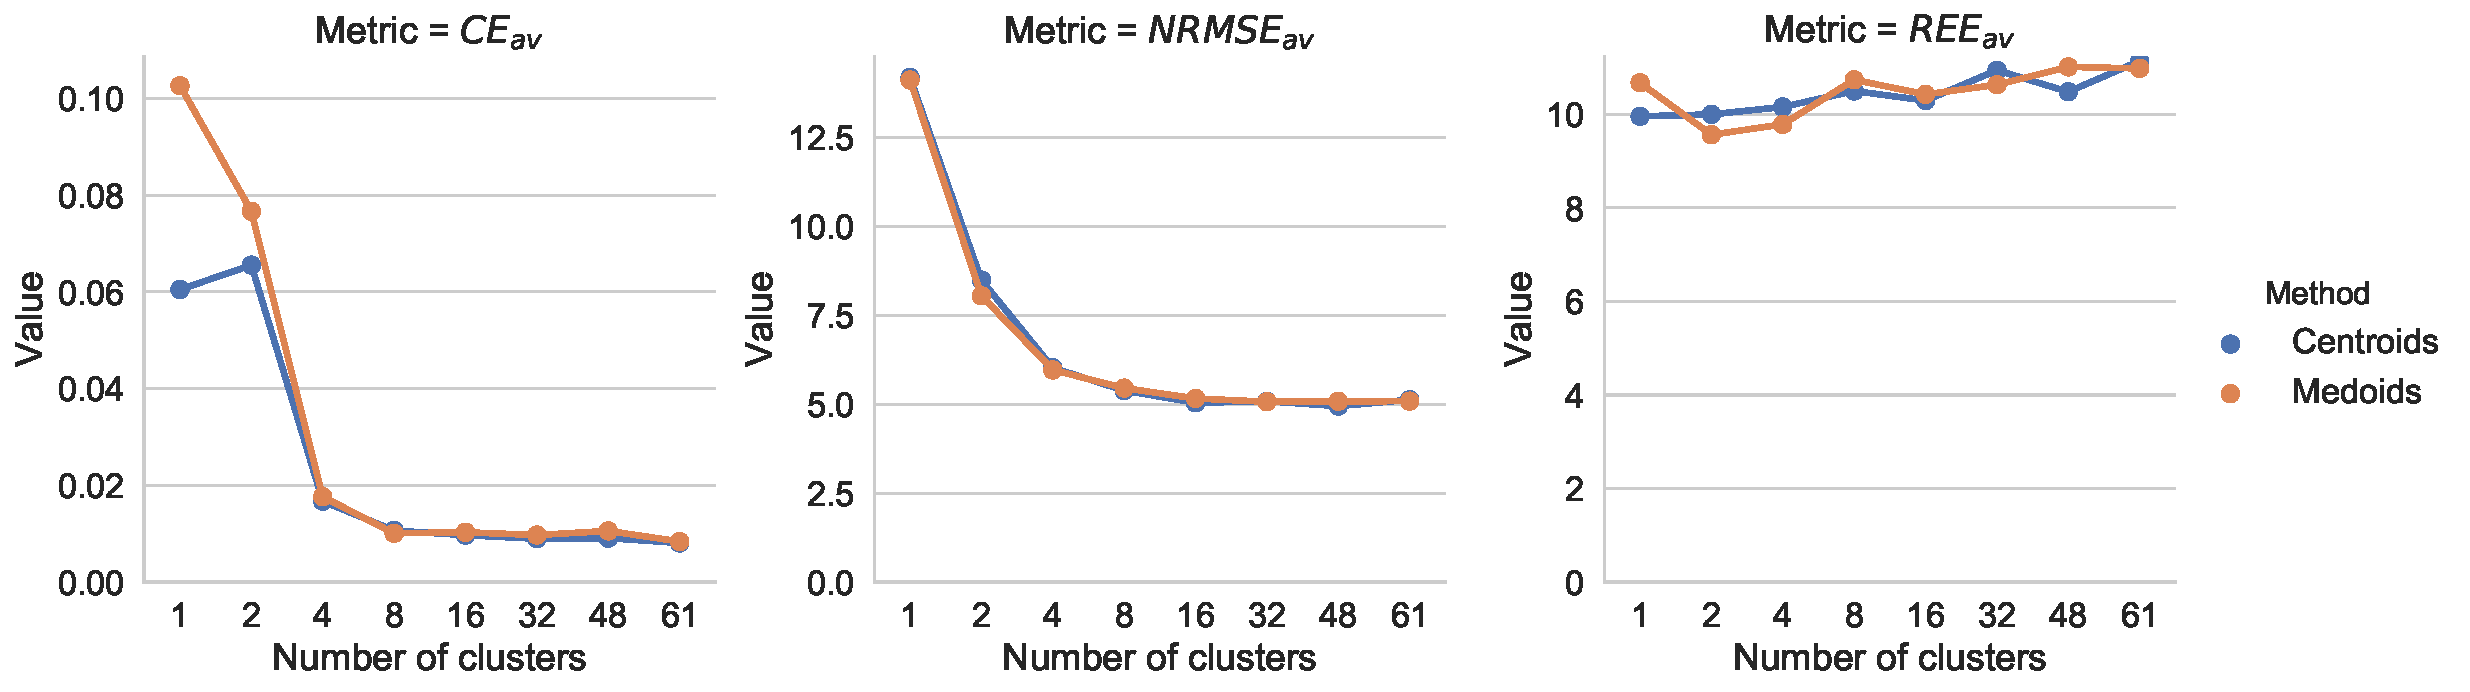
\includegraphics[width=\textwidth]{figures/methods_and_materials/clusters_compared.pdf}
\caption{Comparison of number of clusters for accuracy.}
\label{fig:clusters_compared}
\end{figure*}

The error metrics do not exhibit a significant difference between using either the centroids or medoids technique. However, we chose to use the medoids technique. This was done due to the fact that the extreme high and low values would not be lost due to averaging \cite{Hilbers2019}.

Figure \ref{fig:clusters_compared_load} and Figure \ref{fig:clusters_compared_resources} display the resultant representative days that were used to represent an entire year in the simulation. A positive correlation between onshore and offshore wind speed can be seen in Figure \ref{fig:clusters_compared_resources}, which one would expect for the relatively small geography of the United Kingdom. Between the hours of 96 and 120 a negative correlation of solar irradiance and wind speed is exhibited, which may refer to a particularly sunny and windless day. Whereas between 72 and 96 a particularly windy and sunless day is exhibited.

\begin{figure}
\centering
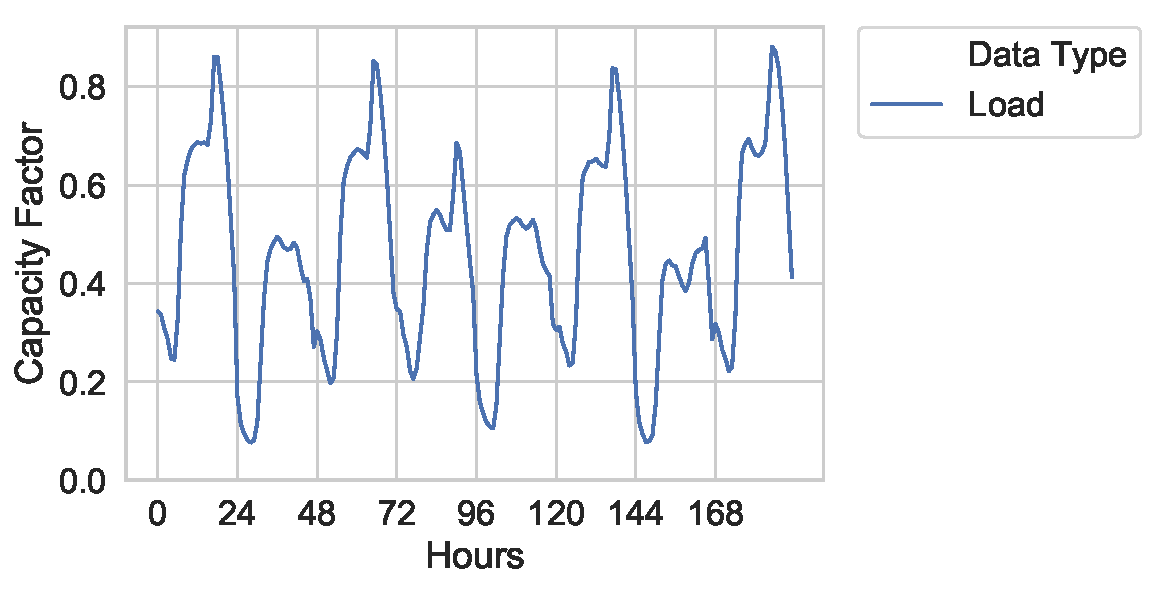
\includegraphics[width=0.49\textwidth]{figures/methods_and_materials/clusters_results_load.pdf}
\caption{Representative days of electricity demand.}
\label{fig:clusters_compared_load}
\end{figure}

Figure \ref{fig:clusters_compared_load} refers to the electrical load of the representative days. It should be noted that these representative days represent a quasi-temporal year and do not represent actual months.


\begin{figure}
\centering
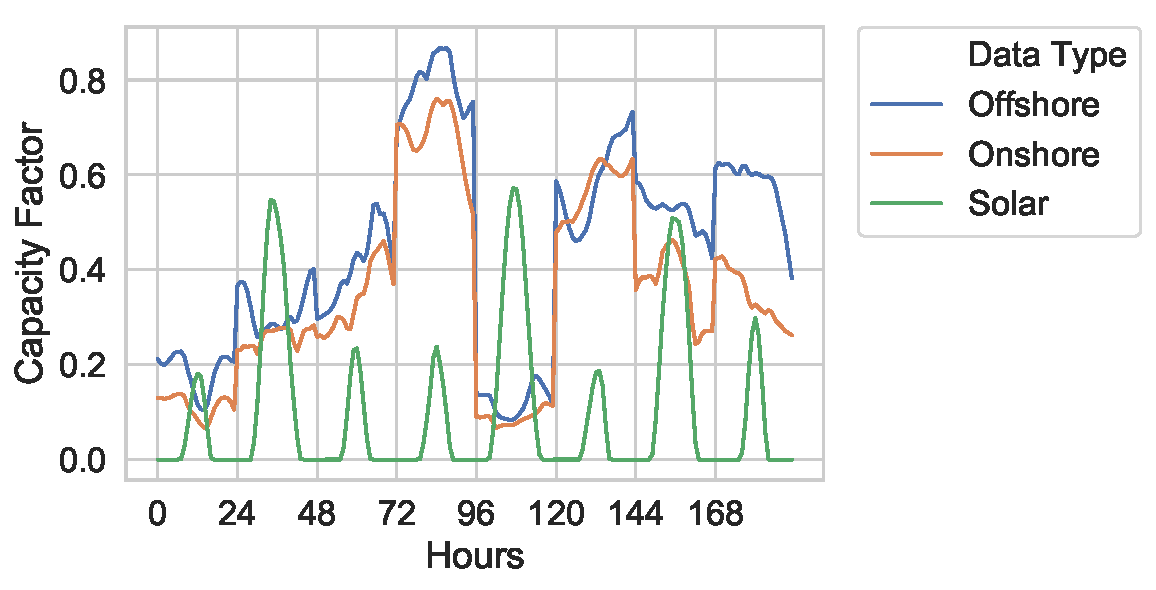
\includegraphics[width=0.49\textwidth]{figures/methods_and_materials/clusters_results_resources.pdf}
\caption{Representative days of renewable resources.}
\label{fig:clusters_compared_resources}
\end{figure}


\subsection{Integrating higher temporal granularity}

To integrate the additional temporal granularity of the model, extra time-steps were taken per year. In this scenario we modelled a single year as 8 days. This enabled us to reduce computational runtime, whilst approximating an entire year.

GenCos make bids at the beginning of every time-step (day) and the Power Exchange matches demand with supply in merit-order dispatch using the previously mentioned uniform pricing market in Section \ref{sec:power_exchange}. An example day is shown in Figure \ref{fig:single_dispatched_day}. 

Figure \ref{fig:single_dispatched_day} displays the high utilization of low marginal-cost generators such as nuclear, wind and photovoltaics. At hour 19, an increase in offshore wind leads to a direct decrease in CCGT. In contrast to this, a decrease in offshore and onshore between the hours of 8 and 12 lead to an increase in dispatch of coal and CCGT. This is behaviour which one would expect to prevent blackouts and meet demand at all times. This process has enabled us to more closely match fluctuations in IRES.

\begin{figure}
\centering
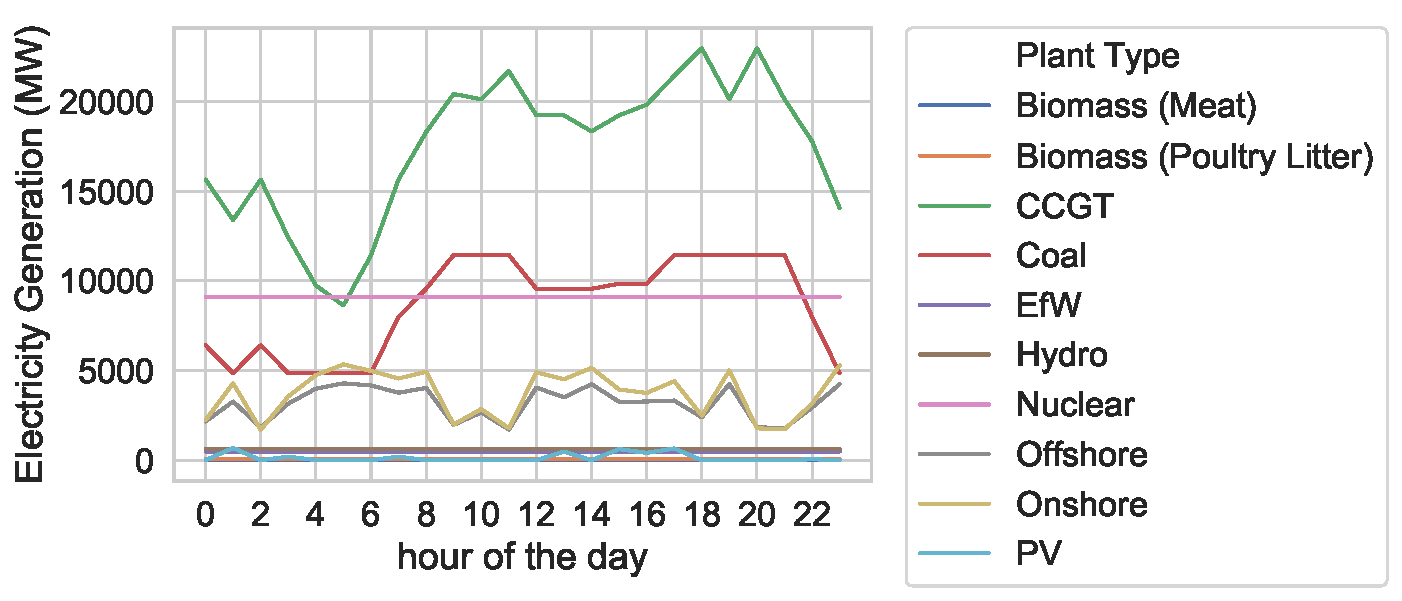
\includegraphics[width=0.49\textwidth]{figures/methods_and_materials/clusters_results_single_day.pdf}
\caption{Example of a single day of dispatched supply.}
\label{fig:single_dispatched_day}
\end{figure}
 
\subsection{Problem Formulation}

For GenCos to adequately make investments they must formulate an expectation of future electricity prices over the lifetime of a plant. Future electricity prices are a function of demand and supply, and with renewable electricity generator costs falling future prices are uncertain \cite{IRENA2014}. 

Due to the uncertainty of future electricity prices over the horizon of the lifetime of a power plant we have set future electricity prices as an exogenous variable that can be set by the user in ElecSim.

To verify the accuracy of ElecSim we used a simple genetic algorithm approach to find the optimum price duration curve in the form of a linear regression model. We validated between the years of 2013 and 2018.

Equation \ref{eq:problem_formulation} details this formally.

\begin{equation}
	\label{eq:problem_formulation}
	minimize \sum\limits_{o\in O}\left(
	\frac{\left|A_o-S_o\right|}
	{\left|\left|O\right|\right|}
	\right)
\end{equation}

Where $o\in O$ refers to the percentage electricity mix output for wind (offshore $+$ onshore generation), nuclear, solar, CCGT, and coal for the year 2018. $A_o$ refers to actual electricity mix for 2018 and $S_o$ refers to simulated electricity mix.

We compared our higher granularity time-step results with a time-step of 20 steps per year, in comparison to 192 time-steps per year using representative days.

\subsection{Genetic Algorithms}

Genetic Algorithms (GAs) are a type of evolutionary algorithm. In this section we detail the genetic algorithm used in this paper.

Initially, a population $P_{0}$ is generated for generation 0. Each of these populations are evaluated for their fitness. A subset of these individuals $C_{t+1} \subset P_{t}$ are chosen for mating. This subset is selected proportionally to their fitness. With `Fitter' individuals having a higher change of reproducing to create the offspring group $C'_{t+1}$. $C'_{t+1}$ have characteristics dependent on the genetic operators: crossover and mutation. The genetic operators are an implementation decision \cite{FogelDavidB2009}. 

Once the new population has been created, the new population $P_{t+1}$ is created by merging individuals from $C'_{t+1}$ and $P_{t}$. See Algorithm \ref{genetic-algorithm} for detailed pseudocode.
%
\begin{algorithm}[t]
\begin{algorithmic}[1]
\State $t=0$
\State initialize $P_{t}$
\State evaluate structures in $P_{t}$
\While {termination condition not satisfied}
\State $t=t+1$
\State select reproduction $C_{t}$ from $P_{t-1}$
\State recombine and mutate structures in $C_{t}$

forming $C'_{t}$
\State evaluate structures in $C'_{t}$
\State select each individual for $P_{t}$ from $C'_{t}$ 

or $P_{t-1}$
\EndWhile
\caption{Genetic algorithm \cite{FogelDavidB2009}}
\label{genetic-algorithm}
\end{algorithmic}
\end{algorithm}



\begin{itemize}
	\item Reproducible data
	\item Summarize previously published results
	\item Modifications of previous results for this paper
\end{itemize}

\section{Results}
\label{sec:results}


\subsection{Validation results and comparison}


Figure \ref{fig:actual_vs_simulated_validation} shows the simulated electricity mix compared to the actual electricity mix between the years of 2013 to 2018 for the best price duration parameter set.


\begin{figure}
\centering
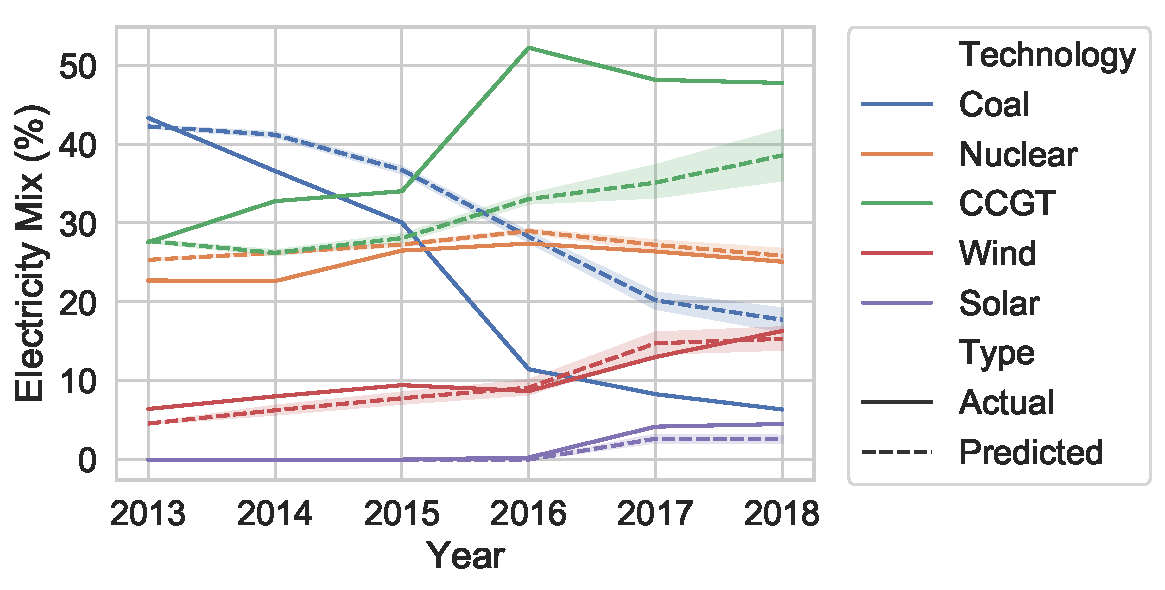
\includegraphics[width=0.49\textwidth]{figures/results/throughout_years.pdf}
\caption{Electricity mix actual vs. simulated for validation scenario with eight representative days.}
\label{fig:actual_vs_simulated_validation}
\end{figure}


Figure \ref{fig:best_price_curve} displays the predicted price duration curve used by the GenCos to achieve the most optimal electricity mix. Where the black line is the price duration curve simulated in 2018, and the red line is the optimal predicted electricity mix. 

The optimal predicted electricity mix closely matches the simulated fit in 2018 with a realistic price duration curve, shown by Figure \ref{fig:best_price_curve}.

The optimal predicted price duration curve has a slightly higher peak price and lower baseload price. This could be due to the fact that there is an increase in the number of renewables with a low SRMC. However, due to the intermittency of renewables such as solar and wind, higher peak prices are required to generate in the times of low wind and sunny days.

\begin{figure}
\centering
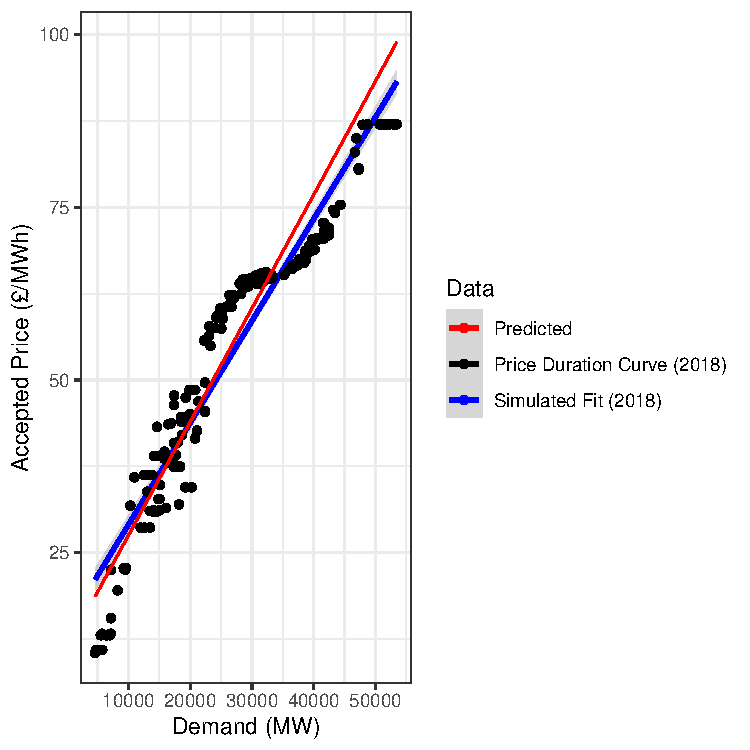
\includegraphics[width=0.49\textwidth]{figures/results/best_run_price_dur_curve.pdf}
\caption{Predicted price curve for investment for most accurate run against simulated run in 2018.}
\label{fig:best_price_curve}
\end{figure}


Figure \ref{fig:actual_vs_simulated_validation} shows a rapid uptakes in solar and wind from the year of 2016, which closely matches the actual uptake. As well as this, the actual mix displays a rapid transition from coal to CCGT. Whilst ElecSim matches this trend, it is not matched precisely. 

Figure \ref{fig:uk_validated_results_2018} compares the electricity mix in the year 2018 for actual and simulated by ElecSim for the optimal predicted price duration curve. 

\begin{figure}
\centering
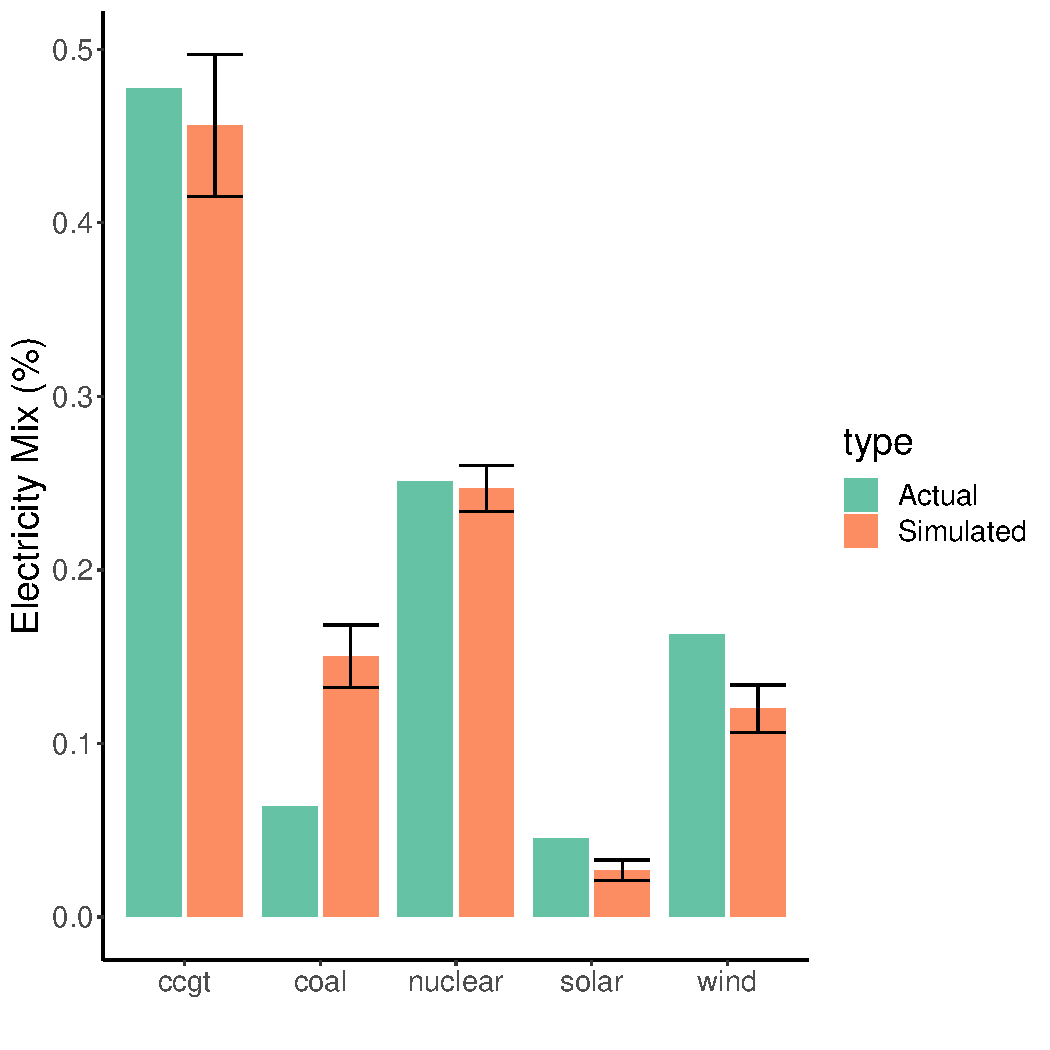
\includegraphics[width=0.45\textwidth]{figures/results/best_run.pdf}
\caption{Electricity generation transition from 2013 to 2018 in the United Kingdom.}
\label{fig:uk_validated_results_2018}
\end{figure}


We compare our projections from 2013 to 2018 with the UK Governments (BEIS) projections made in 2013 in Figure \ref{fig:beis_elecsim_historic_comparison} \cite{UKDECC2013}. BEIS were also unable to precisley match the transition from coal to CCGT. However, they were able to model the large transition of coal to CCGT in the year 2016.

However, the BEIS projection overestimates the uptake in renewables in the year 2016, which ElecSim does not.


\begin{figure}
\centering
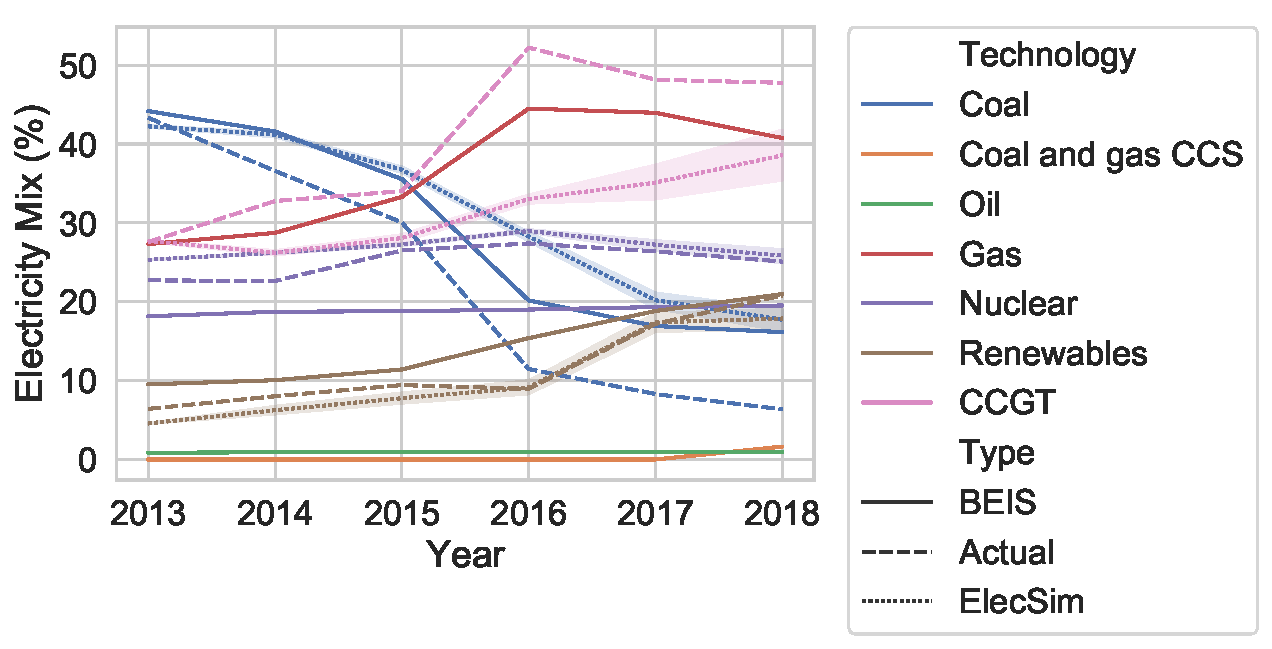
\includegraphics[width=0.49\textwidth]{figures/results/throughout_years_beis_elecsim_comparison.pdf}
\caption{Comparison of actual electricity mix vs. ElecSim vs. BEIS projections.}
\label{fig:beis_elecsim_historic_comparison}
\end{figure}

We display the error metrics to evaluate our models 5 year projections in table \ref{table:metrics}. Where MAE is mean absolute squared error, MASE is mean absolute scaled error, RMSE is root mean squared error, and SD is standard deviation.

We are able to improve the projections for all but nuclear based on the naive forecasting approach using ElecSim. Where in the naive approach we predict the next time-step by using the last known time-step. 


\begin{table}[htb]
    \centering
\csvautobooktabular{table_data/results/error_metrics.csv}
    \caption{Error metrics for time series forecast from 2013 to 2018}
    \label{table:metrics}
\end{table}

Figure \ref{fig:single_time_step_results} displays the results using the same scenario details such as fuel and carbon price, electricity generation costs and GenCos. As mentioned in Section \ref{ssec:representative_days}, we see an overestimation in the uptakes of IRES. In this case all electricity sources are replaced by wind which with current storage technologies is not possible.



\begin{figure}
\centering
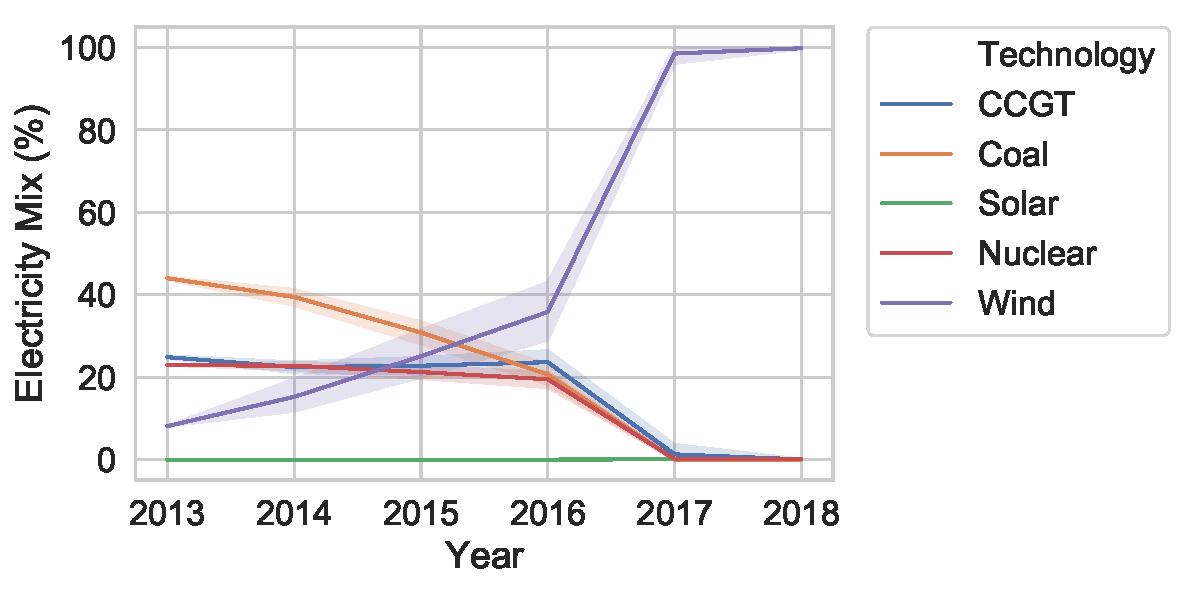
\includegraphics[width=0.49\textwidth]{figures/results/yearly_time_step_scenario.pdf}
\caption{Electricity mix actual vs. simulated for validation scenario with a single representative day.}
\label{fig:single_time_step_results}
\end{figure}











\begin{itemize}
	\item Clear and concise results
\end{itemize}

\section{Discussion}
\label{sec:discussion}

\begin{itemize}
	\item Significance of work
	\item Avoid discussion of public work
\end{itemize}

\section{Conclusion}
\label{sec:conclusion}

\begin{itemize}
	\item Main conclusions
\end{itemize}

\section{Funding Sources}

This work was supported by the Engineering and Physical Sciences Research Council, Centre for Doctoral Training in Cloud Computing for Big Data [grant number EP/L015358/1].




%% The Appendices part is started with the command \appendix;
%% appendix sections are then done as normal sections
%% \appendix

%% \section{}
%% \label{}

%% If you have bibdatabase file and want bibtex to generate the
%% bibitems, please use
%%
  \bibliographystyle{elsarticle-num} 
  \section*{References}
  \bibliography{library,bib_custom}

%% else use the following coding to input the bibitems directly in the
%% TeX file.

%\begin{thebibliography}{00}
%
%%% \bibitem[Author(year)]{label}
%%% Text of bibliographic item
%
%\bibitem[ ()]{}
%
%\end{thebibliography}
\end{document}

\endinput
%%
%% End of file `elsarticle-template-harv.tex'.
	